\documentclass[11pt,spanish]{book}

\usepackage{amsmath}
\usepackage{amsthm}
\usepackage[spanish]{babel}
\usepackage{amssymb}
\usepackage{mathtools}
\usepackage{multirow}
\usepackage{colortbl}
\usepackage{color}
\usepackage{multicol}
\usepackage{float}
\usepackage{biblatex}
\newtheorem{definition}{Definition}[section]
\newtheorem{lemma}{Definition}[section]
\newtheorem{example}{Definition}[section]
\newtheorem{theorem}{Definition}[section]
\DeclareMathOperator{\tr}{Tr}
\DeclareMathOperator{\diag}{Diag}
\newcommand{\matr}[1]{\mathbf{#1}}
\providecommand{\tq}{\mid}
\providecommand{\N}{\mathbb{N}}
\providecommand{\Z}{\mathbb{Z}}
\providecommand{\Q}{\mathbb{Q}}
\providecommand{\R}{\mathbb{R}}
\providecommand{\C}{\mathbb{C}}
\providecommand{\H}{\mathcal{H}}
\providecommand{\Im}[1]{Im(#1)}
\providecommand{\Re}[1]{Re(#1)}
\let\oldforall\forall
\renewcommand{\forall}{\oldforall\,}
\let\oldexists\exists
\renewcommand{\exists}{\oldexists\,}
\newcommand{\existsUnique}{\oldexists!\,}
\providecommand{\conjugate}[1]{\bar{#1}}
\providecommand{\pescalar}[2]{\langle #1,#2 \rangle}
\providecommand{\braket}[2]{\left\langle#1\mid#2\right\rangle}
\providecommand{\bra}[1]{\left\langle#1\right\rvert}
\providecommand{\ket}[1]{\left\lvert#1\right\rangle}
\providecommand{\ketbra}[2]{\left\lvert#1\right\rangle\!\left\langle#2\right\rvert}
\providecommand{\so}{\Rightarrow}
\renewcommand{\iff}{\Leftrightarrow}
\providecommand{\by}[1]{\overset{\fbox{\tiny #1}}{=}}
\providecommand{\byref}[1]{\overset{\fbox{\tiny\ref{#1}}}{=}}
\providecommand{\maps}[3]{#1:#2\longrightarrow #3}
\providecommand{\coma}{,\thinspace}
\providecommand{\pari}[2]{(#1,\thinspace #2)}
\providecommand{\indexdots}[3]{#1=#2,\ldots,#3}
\providecommand{\define}[2]{\textbf{#1}\label{def:#2}}
\providecommand{\avg}[1]{\left\langle#1\right\rangle}
\providecommand{\abs}[1]{\lvert#1\rvert}
\providecommand{\nor}[1]{\lVert#1\rVert}
\providecommand{\operatoravg}[3]{\left\langle#1|#2|#3\right\rangle}
\newcommand{\set}[1]{\left\{#1\right\}}
\newcommand{\where}{\mathrel{}\middle|\mathrel{}}
\newcommand{\lista}[2]{#1\coma \dots \coma #2}
\newcommand{\ndots}[3]{#1 = #2\coma \dots \coma #3}
%Kets notables
\newcommand{\ketMas}{\frac{1}{\sqrt{2}}(\ket{0}+\ket{1})}
\newcommand{\ketMenos}{\frac{1}{\sqrt{2}}(\ket{0}-\ket{1})}
\newcommand{\ketIMas}{\frac{1}{\sqrt{2}}(\ket{0}+i\ket{1})}
\newcommand{\ketIMenos}{\frac{1}{\sqrt{2}}(\ket{0}-i\ket{1})}
\newcommand{\ketBellUno}{\frac{1}{\sqrt{2}}(\ket{00}+\ket{11})}
\newcommand{\ketBellDos}{\frac{1}{\sqrt{2}}(\ket{00}-\ket{11})}
\newcommand{\ketBellTres}{\frac{1}{\sqrt{2}}(\ket{10}+\ket{01})}
\newcommand{\ketBellCuatro}{\frac{1}{\sqrt{2}}(\ket{10}-\ket{01})}

%OPERADORES 2x2
\newcommand{\matrixX}{\begin{pmatrix}
	                      0 & 1 \\ 1 & 0
\end{pmatrix}}
\newcommand{\matrixY}{\begin{pmatrix}
	                      0 & -i \\ i & 0
\end{pmatrix}}
\newcommand{\matrixZ}{\begin{pmatrix}
	                      1 & 0 \\ 0 & -1
\end{pmatrix}}
\newcommand{\matrixH}{\frac{1}{\sqrt {2}}  \begin{pmatrix}
	                                           1 & 1 \\ 1 & -1
\end{pmatrix}}
%OPERADORES $4x4
\newcommand{\matrixCNOT}{\begin{pmatrix}
	                         1 & 0 & 0 & 0 \\ 0 & 0 & 0 & 1 \\ 0 & 0 & 1 & 0 \\ 0 & 1 & 0 & 0
\end{pmatrix}}
\providecommand{\logical}[2]{#1_{\shortrightarrow #2}}
\providecommand{\logicalGeneric}[1]{\logical{#1}{n}}
\providecommand{\palabra}[2]{#1_1\cdots #1_{#2}}
\providecommand{\palabraN}[1]{\palabra{#1}{n}}
\providecommand{\palabraG}{\palabra{x}{n}}
\providecommand{\push}[1]{\stackrel{\hookrightarrow}{#1}}
\providecommand{\pull}[1]{\stackrel{\hookleftarrow}{#1}}
\providecommand{\lowerInt}[1]{\lfloor #1 \rfloor}
\providecommand{\upperInt}[1]{\lceil #1 \rceil}
\providecommand{\mas}{\oplus}
\providecommand{\menos}{\circleddash}
\providecommand{\por}{\otimes}
\providecommand{\Rr}[2]{\updownarrow_{#1, #2}}
\providecommand{\Rrr}[2]{\circlearrowleft_{#1, #2}}
\providecommand{\Rrrr}[3]{\updownarrow_{#1, #2, #3}}
\providecommand{\Cc}[2]{\leftrightarrow^{#1, #2}}
\providecommand{\Ccc}[2]{\circlearrowleft^{#1, #2}}
\usepackage[left=1.75cm,
	right=1.5cm,
	top=3.52cm,
	bottom=3.23cm]{geometry}
\usepackage{fancyhdr}
\usepackage{graphicx}
\usepackage{sectsty}
\usepackage{titlesec}
\setlength{\parskip}{\baselineskip}
\newcommand{\personalheader}[2]{
	\pagestyle{fancy}
  \setlength{\headsep}{50pt}
  \setlength{\footskip}{13.866141732pt}
	\setlength{\headheight}{38.87935pt}
	\addtolength{\topmargin}{-26.87935pt}
	\renewcommand{\headrulewidth}{0pt}
	\fancyhead[R]{#1\\\ \\#2}
	\fancyfoot{}
	\fancyfoot[R]{\thepage}
}
\newcommand{\titulo}[1]{\textcolor{unir-azul-fuerte}{\LARGE{\textbf{#1}}}\vspace{0.1in}}
\titleformat{\chapter}[hang]{\vspace{-4cm}\huge\bfseries\color{unir-azul-fuerte}}{\thechapter. }{0pt}{\Huge\bfseries}
\newcommand{\primersubtitulo}[1]{\textcolor{unir-azul-fuerte}{\large #1}}
\newcommand{\subtitulo}[1]{\vspace{0.1in}\textcolor{unir-azul-fuerte}{\large #1}}
\newcommand{\seccion}[1]{\vspace{0.1in}\textbf{#1}}
\renewcommand{\labelitemi}{$\textcolor{unir-azul-fuerte}{\bullet}$}
\renewcommand{\labelitemii}{$\textcolor{unir-azul-fuerte}{\cdot}$}
\renewcommand{\labelitemiii}{$\textcolor{unir-azul-fuerte}{\diamond}$}
\renewcommand{\labelitemiv}{$\textcolor{unir-azul-fuerte}{\ast}$}
\chapterfont{\color{unir-azul-fuerte}}
\sectionfont{\color{unir-azul-fuerte}}
\subsectionfont{\color{unir-azul-fuerte}}
\renewcommand*\contentsname{\textcolor{unir-azul-fuerte}{Índice de contenidos}}
\renewcommand{\listfigurename}{\textcolor{unir-azul-fuerte}{Índice de figuras}}
\renewcommand{\listtablename}{\textcolor{unir-azul-fuerte}{Índice de tablas}}
\begin{document}
	\frontmatter
	\personalheader{Gustavo Recalde Vásquez}{Algoritmos Cuánticos para optimzacion de Rutas}
	\begin{center}
	
\includegraphics[width=10.6cm,height=2.88cm]{logo}

	\Huge Universidad Internacional de La Rioja

	\huge Escuela Superior de Ingeniería y \\ Tecnología

	\vspace{100pt}

	\LARGE Máster Universitario en Computación Cuántica

	\Huge \textcolor{unir-azul-fuerte}{Algoritmos cuánticos para optimización de rutas}
	\normalsize

	\vspace{100pt}

\end{center}
\begin{tabular}{ll}
	Trabajo Fin de Master & \\
	\textbf{presentado por:} Gustavo Recalde Vásquez & \\
	\textbf{Director/a:} Francisco Costa Cano & \\
	\textbf{Fecha:} 30 junio de 2024 & \\
\end{tabular}
	\chapter{Resumen}

En este apartado se introducirá un breve resumen en español del trabajo realizado (extensión máxima: 150 palabras). Este resumen debe incluir el objetivo o propósito de la investigación, la metodología, los resultados y las conclusiones.

{\bf Palabras clave:} se deben incluir de 3 a 5 palabras claves en español
	\titulo{Abstract}

En este apartado se introducirá un breve resumen en inglés del trabajo realizado. Este resumen debe incluir el objetivo o propósito de la investigación, la metodología, los resultados y las conclusiones.

(Aproximadamente 150 palabras)

\textbf{Keywords:} (De 3 a 5 palabras en inglés)
	\tableofcontents
	\listoffigures
	\listoftables
	\mainmatter
	\chapter{Introducción}

Este trabajo se centra en el desarrollo y aplicación de algoritmos cuánticos para la optimización de rutas de entrega y volumen de carga en la empresa Wolf. Utilizando técnicas de computación cuántica, se busca abordar los desafíos específicos relacionados con la eficiencia en la distribución y el aprovechamiento del espacio de carga en una flota de camiones. 

%El primer capítulo es siempre una introducción. En ella debes resumir de forma esquemática pero suficientemente clara lo esencial de cada una de las partes del trabajo. La lectura de este primer capítulo ha de dar una primera idea clara de lo que se pretendía, las conclusiones a las que se ha llegado y del procedimiento seguido.
%Como tal, es uno de los capítulos más importantes de la memoria. Las ideas principales a transmitir son la identificación del problema a tratar, la justificación de su importancia, los objetivos generales (a grandes rasgos) y un adelanto de la contribución que esperas hacer.
%Típicamente una introducción tiene tres apartados: Motivación, Planteamiento del trabajo, Estructura del trabajo. (Texto Normal del menú de estilos.)
%(Ejemplo de nota al pie\footnote{Ejemplo de nota al pie.}.)

\section{Motivación}

    El transporte y la logística son vitales para la economía global, pero enfrentan problemas significativos relacionados con la optimización de rutas y la carga de vehículos. Las soluciones actuales son a menudo ineficientes, llevando a un uso subóptimo de recursos, aumento de costos y tiempo de entrega. Este trabajo identifica y aborda estas ineficiencias utilizando algoritmos cuánticos, que prometen una capacidad superior para manejar la complejidad y dinamismo de tales sistemas.
    La importancia de optimizar rutas de entrega y carga se magnifica en contextos de alta demanda y diversidad geográfica, como lo es el caso de la empresa Wolf. Los desafíos incluyen la gestión eficiente de múltiples puntos de recolección y distribución, la variabilidad en el tamaño y volumen de los paquetes, y restricciones temporales estrictas. La computación cuántica ofrece un enfoque prometedor para superar estos retos, lo que podría resultar en una significativa reducción de costos operativos y mejora en la eficiencia del servicio.


%Cuál es el problema que quieres tratar? ¿Cuáles crees que son las causas? ¿Por qué es relevante el problema?

%A continuación, se indica con un ejemplo cómo deben introducirse los títulos y las fuentes en Tablas y Figuras.

%\begin{table}[t]
%	\begin{center}
%	\caption{Ejemplo de tabla con sus principales elementos.}
%	\label{tab:1}
%	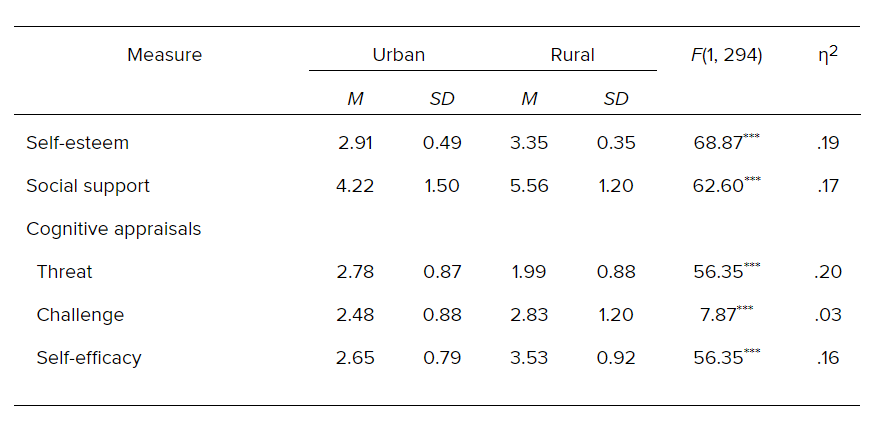
\includegraphics[width=4.90737in,height=2.42708in]{tabla}
%	\small Fuente: American Psychological Association, 2020e.
%	\end{center}
%\end{table}

%\begin{figure}[H]
%	\begin{center}
%		\caption{Ejemplo de figura realizada para nuestro trabajo.}
%		\label{fig:1}
%		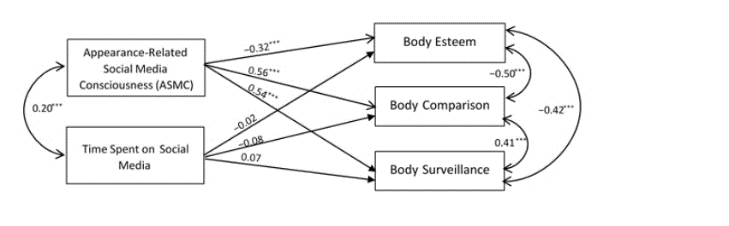
\includegraphics[width=4.90737in,height=2.42708in]{figura}
%%		\small Fuente: American Psychological Association, 2020f.
%	\end{center}
%\end{figure}

\section{Planteamiento del trabajo}

    Este estudio se centra en el desarrollo y evaluación de algoritmos cuánticos diseñados para optimizar las rutas de entrega y la carga de camiones para la empresa Wolf. Se analizarán y compararán estos algoritmos con métodos clásicos de optimización para determinar su viabilidad y eficacia. Dividiremos el probleam en tres partes específicos:

    \begin{itemize}
    \item Optimización de rutas: Desarrollar un algoritmo que mejore la eficiencia de las rutas de entrega, teniendo en cuenta la ubicación geográfica de los puntos de distribución, el tamaño y volumen de los paquetes, y los intervalos de tiempo de entrega.
    
    \item Planificación de itinerarios: Crear un sistema que detalle el tiempo estimado de llegada para cada vehículo a todos los puntos de distribución.
    
    \item Optimización de la carga: Mejorar el proceso de carga de los vehículos, ordenando los paquetes de manera que se maximice el uso del espacio disponible y se optimice la eficiencia del transporte.
    
    La investigación evaluará la aplicabilidad de varios algoritmos cuánticos, incluyendo el recocido cuántico y el algoritmo de Grover, y utilizará plataformas como IBM Quantum, D-Wave y Rigetti.
    \end{itemize}

%¿Cómo se podría solucionar el problema? ¿Qué es lo que se propone? Aquí describes tu objetivo en términos generales. 

\section{Estructura de la memoria}

    Este trabajo estará organizado en los siguientes capítulos para abordar de manera sistemática el problema de investigación:

    \textbf{Introducción:} Presentación del problema, justificación y objetivos del estudio.
    Fundamentos Teóricos: Explicación de los conceptos básicos de la mecánica cuántica y la computación cuántica necesarios para entender los algoritmos utilizados.
    
    \textbf{Metodología:} Detalle de las técnicas y herramientas cuánticas seleccionadas, así como la metodología de comparación con sistemas clásicos.
    Desarrollo de Algoritmos y Simulaciones: Diseño de los algoritmos cuánticos y realización de simulaciones para evaluar su rendimiento.
    
    \textbf{Resultados y Análisis:} Presentación y análisis de los resultados obtenidos, comparando las soluciones cuánticas con las clásicas.
    
   \textbf{ Conclusiones y Recomendaciones:} Síntesis de los hallazgos y sugerencias para futuras investigaciones o aplicaciones prácticas. 

%Aquí describes brevemente lo que vas a contar en cada uno de los capítulos siguientes.
	\chapter{Contexto y estado del técnica}

Después de la introducción, se suele describir el contexto de aplicación. En este Capítulo debemos mostrar un sobrado conocimiento de la materia, plagando absolutamente TODO lo que mencionemos con referencias. Práticamente, cada frase puede necesitar de alguna referencia.

Las referencias NO están solo para aparentar. Rendimos tributo y reconocemos a las personas que han pensado los problemas antes que nosotros. Puede haber varias referencias válidas para una misma afirmación, y no pasa nada porque así se indique.

Recuerda que para citar trabajos de diferentes autores es fundamental e imprescindible seguir el formato APA, según se describe en el documento Normativa\_APA.pdf disponible en el apartado de Documentación del Aula de información general del Máster Universitario en Computación Cuántica (MUCC). No se debe mencionar, ni utilizar ninguna fuente, sin citarla apropiadamente.

EJEMPLO DE CITAS: Si queremos citar a alguien, por ejemplo porque vamos a hablar de Latex \citep{lamport1994} o porque, según las ideas de \cite{ackerman2017}, la liga de fútbol inglesa debe tener torneos de desempate, pues tenemos que hacerlo correctamente. {\bf{(Ver en la sección Bibliografía cómo deben incluirse las entradas bibliográficas).}}

Este Capítulo puede tener secciones diferentes a las que se indican a continuación, que se indican a modo de ejemplo.

\section{Antecedentes históricos}

En 1980, Paul Benioff propone la primera versión teórica de una máquina de Turing cuántica poniendo de manifiesto que la computación cuántica era, en efecto, teóricamente posible (Benioff, 1980). Poco tiempo después, Richard Feynman constató que existían ciertos fenómenos cuya simulación requería de recursos que crecían de manera exponencial con la complejidad del problema y sugirió el empleo de computadores cuánticos para simular este tipo de fenómenos (Feynman, 1982). A mediados de los 80, David Deustch describe la Máquina de Turing Universal Cuántica, probando que construir un computador cuántico era teóricamente posible (Deutsch, 1985). En este mismo artículo, aparece el algoritmo de Deutsch, el primer algoritmo que resuelve un problema de manera más eficiente que su versión clásica.

Durante la década de los 90, aparecerán dos de los algoritmos más importantes en computación cuántica. En primer lugar, el algoritmo de Shor es capaz de factorizar enteros con una ventaja exponencial respecto a los algoritmos clásicos (Shor, 1994). En segundo lugar, el algoritmo de Grover diseñado para realizar búsquedas en una base de datos no estructurada de manera más eficiente (Grover, 1996). La aparición de estos algoritmos pone de manifiesto la existencia de una ventaja cuántica en este nuevo modelo de computación.

Este nuevo paradigma no utiliza bits clásicos  si no bits cuánticos o qubits, término atribuido a Benjamin Schumacher (1995). En el año 2000, Divincenzo propone 5 requisitos que debe cumplir todo sistema para que pueda ser considerado como una implementación física válida de un computador cuántico (Divincenzo, 2000):

\begin{enumerate}
    \item Debe tratarse de un sistema escalable con al menos un qubit bien caracterizado.
    \item Debe poder inicializarse a un estado inicial, habitualmente 
    $ | 0 \rangle $.
    \item Cada qubit debe tener un tiempo de decoherencia significativamente superior a los tiempos de actuación de las puertas cuánticas.
    \item Debe poseer un conjunto universal de puertas cuánticas.
    \item Debe poseer algún mecanismo que permite medir el estado de los qubits.
\end{enumerate}










\section{Estado actual}

En la siguiente sección, se expondrán todos aquellos conceptos de la Mecánica Cuántica y, mas específicamente, de la computación cuántica de los que nos serviremos durante el desarrollo del presente trabajo.

\subsection{Postulados de la mecánica cuántica}

El formalismo matemático de la mecánica cuántica se rige por los siguientes postulados (Nielsen y Chuang, 2010):

\begin{description}
    \item[Postulado 1] Para cada sistema físico, existe un espacio vectorial complejo con producto interno (es decir, un espacio de Hilbert) conocido como espacio de estado. El estado de dicho sistema queda completamente descrito por un vector unitario perteneciente al espacio de estados. 
    
    \item[Postulado 2] El estado de un sistema evoluciona según una transformación unitaria. Es decir, sea el estado $ | \psi \rangle$ y la transformación unitaria definida por el operador unitario $U$, entonces el estado $ | \psi \rangle $ evolucionará al estado $ | \psi' \rangle = U | \psi \rangle$.
    \item[Postulado 3] Las medidas cuánticas están descritas por un conjunto $ \left \{ M_m \right \}  $ de operadores de medida donde los subíndices $m$ hacen referencia al resultado obtenido en cada medida. Si el sistema se encuentra en el estado $ | \psi \rangle $ en el instante inmediatamente anterior a la medida, entonces la probabilidad de obtener el resultado $m$ es $$ p(m)= \langle \psi | M_m^\dagger M_m | \psi \rangle $$ y el estado del sistema tras la medida será $$ \frac{M_m | \psi \rangle}{\sqrt{\langle \psi | M_m^\dagger M_m | \psi \rangle}} . $$
    \item[Postulado 4] El espacio de estados correspondiente a un sistema físico compuesto viene dado por el producto tensorial de los espacios de estados correspondientes a cada uno de los sistemas físicos que componen nuestro sistema, es decir, $$| \psi \rangle = | \psi_1 \rangle \otimes | \psi_2 \rangle \otimes ... \otimes | \psi_n \rangle .$$
\end{description}

\subsection{Qubit}

Matemáticamente, un qubit es un vector unitario perteneciente a un espacio vectorial complejo de dimensión 2 para el cual existe una base ortonormal determinada por $ \left \{ | 0 \rangle , | 1 \rangle  \right \}$ (Rieffel y Polak, 2000). Así pues, el estado de un qubit queda determinado por cualquier combinación lineal $ | \psi \rangle = \alpha | 0 \rangle + \beta | 1 \rangle $ donde $ \alpha, \beta \in \mathbb{C} $ tal que $ | \alpha |^2 + | \beta |^2=1 $.

Los vectores que forman la base $\{ |0 \rangle , |1 \rangle  \}$ vienen dados por

$$ |0 \rangle = \begin{pmatrix} 1\\ 0 \end{pmatrix}, |1 \rangle = \begin{pmatrix} 0\\ 1 \end{pmatrix}.$$

Existen ciertos estados que, debido a su recurrencia, poseen una denotación propia (Nielsen y Chuang, 2010). Estos estados son los siguientes:

$$ | + \rangle = \frac{1}{\sqrt{2}} | 0 \rangle + \frac{1}{\sqrt{2}} | 1 \rangle $$
$$ | - \rangle = \frac{1}{\sqrt{2}} | 0 \rangle - \frac{1}{\sqrt{2}} | 1 \rangle $$
$$ | i \rangle = \frac{1}{\sqrt{2}} | 0 \rangle + \frac{i}{\sqrt{2}} | 1 \rangle $$
$$ | -i \rangle = \frac{1}{\sqrt{2}} | 0 \rangle - \frac{i}{\sqrt{2}} | 1 \rangle $$

Ya que $ \langle \psi | \psi \rangle = | \alpha |^2 + | \beta |^2=1$, entonces existe $ \theta \in [0, \pi]$ tal que $ | \alpha | = cos ( \frac{\theta}{2} )$ y $ | \beta | = sen ( \frac{\theta}{2} )$. De este modo, el estado de un qubit se puede representar de la siguiente manera

$$ | \psi \rangle = cos ( \frac{\theta}{2}) | 0 \rangle + e^{i \phi} sen ( \frac{\theta}{2} ) | 1 \rangle  $$

donde $\phi \in [0 , 2 \pi)$ representa la fase relativa entre los coeficientes (Willsh, Willsh y Michielsen, 2022).

De la expresión anterior, se sigue que existe una aplicación biyectiva entre cada estado cuántico y la superficie de una esfera tridimensional de radio 1, es decir, el estado cuántico de un qubit puede representarse como un punto sobre la superficie de una esfera de radio igual a 1. Esta representación se conoce como representación sobre la esfera de Bloch (1946).



\begin{figure}[ht]
	\begin{center}
		\caption{Representación sobre la Esfera de Bloch}
		\label{fig:fig-1}
		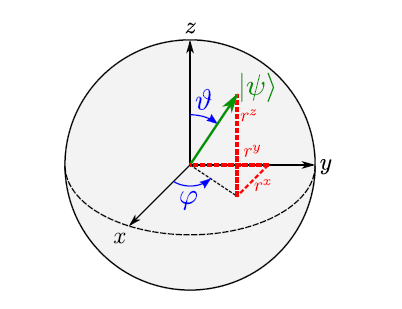
\includegraphics[width=0.5\linewidth]{Bloch.PNG}
		\small Fuente: American Psychological Association, 2020f.
	\end{center}
\end{figure}

\subsection{Medida}

En virtud del postulado 3 de la Mecánica Cuántica, existen dos resultados posibles cuando medimos el estado de un qubit, $ |0 \rangle $ o $ | 1 \rangle$. Sea el estado $ | \psi \rangle = \alpha | 0 \rangle + \beta | 1 \rangle$, entonces como resultado de una medición se obtendrá el estado $| 0 \rangle$ con una probabilidad $ | \alpha|^2$ y el estado $ | 1 \rangle $ con una probabilidad $ | \beta |^2$.

Una importante característica de las medidas cuánticas es que el estado inmediatamente anterior a la medida es destruido y sustituido por el resultado obtenido en la medida. Veamos qué implicaciones tiene esto para la cantidad de información que puede codificarse sobre un único qubit.

Como hemos visto anteriormente, cada estado cuántico se corresponde con un único punto sobre la esfera de Bloch. Dado que la superficie de la esfera tiene infinitos puntos cabría esperar que, en principio, cualquier cantidad de información pudiera ser codificada en un único qubit. No obstante, es necesario prestar atención a la naturaleza intrínseca de las medidas cuánticas ya que solo dos resultados posibles pueden producirse. Dicho de otro modo, de un único qubit mediante una medida, únicamente puede obtenerse un bit de información clásica de su estado (Nielsen y Chuang, 2010).

Otra cuestión interesante respecto a las medidas cuánticas es que pueden realizarse respecto a cualquier a base ortonormal del espacio de Hilbert. Por ejemplo, si se mide un qubit respecto de la base $\{ |+ \rangle, | - \rangle \}$, conocida como base de Hadamard, entonces los posibles resultados serán los estados $ | + \rangle$ y $ | - \rangle $. De esto, se deduce que la superposición cuántica es un fenómeno relativo a la base utilizada. Es decir, si se mide el estado $| + \rangle $ respecto de la base computacional $\{ |0 \rangle, | 1 \rangle \}$, se obtendrá el estado $ | 0 \rangle $ con un 50 $ \% $ de probabilidad o el estado $ | 1 \rangle $ con otro 50 $ \% $ de probabilidad. Queda claro que el estado $ | + \rangle $ encarna una superposición uniforme respecto de la base computacional. Del mismo modo, si se mide el estado $| 1 \rangle $ respecto de la base de Hadamard $\{ |+ \rangle, | - \rangle \}$, se obtendrá el estado $ | + \rangle $ con un 50 $ \% $ de probabilidad o el estado $ | - \rangle $ con otro 50 $ \% $ de probabilidad. Se deduce que el estado $ | 1 \rangle $ presenta una superposición uniforme respecto de la base Hadamard.


	\chapter{Descripción detallada e identificación de requisitos}

%En este capítulo se debe indicar el trabajo previo realizado, detallando el problema a tratar, su contexto y los requisitos.

\section{Contexto del Problema}

La empresa Wolf opera una flota de 15 camiones que distribuyen productos a múltiples puntos de entrega dentro de una amplia región geográfica. La optimización actual de rutas y la carga de los camiones enfrentan desafíos significativos debido a la variabilidad en las demandas de entrega, los diferentes tamaños y volúmenes de los paquetes, y las restricciones de tiempo. Estas ineficiencias resultan en costos operativos elevados y tiempos de entrega prolongados, afectando la competitividad y la sostenibilidad de la empresa.


\section{Identificación de Requisitos}
Para abordar este problema mediante la aplicación de algoritmos cuánticos, se han identificado varios requisitos clave que deben ser satisfechos:

\subsection{Requisitos Funcionales}
Desarrollo de un Algoritmo de Optimización de Rutas Cuántico: Diseñar un algoritmo cuántico que mejore la eficiencia de las rutas de entrega, considerando variables como la geolocalización de los puntos de distribución, el tamaño y volumen de los paquetes, y los intervalos de tiempo preferidos para la entrega.

\begin{itemize}
\item Planificación de Itinerarios Detallados: El sistema debe ser capaz de generar un itinerario detallado que indique el tiempo estimado de llegada de cada camión a todos los puntos de distribución a lo largo de la ruta.

\item Optimización de la Carga del Vehículo: Implementar un método para optimizar el proceso de carga en los vehículos, asegurando que el orden de los paquetes maximice el uso del espacio disponible y mejore la eficiencia del transporte.
\end{itemize}

\subsection{Requisitos No Funcionales}
Eficiencia Computacional: El algoritmo debe ser computacionalmente eficiente para ser ejecutado en plataformas cuánticas disponibles actualmente, como las ofrecidas por IBM Quantum, D-Wave y Rigetti.

\begin{itemize}
\item Escalabilidad: El sistema debe ser escalable para adaptarse a aumentos en el número de vehículos o cambios en la red de distribución.

\item Usabilidad: La interfaz del sistema debe ser intuitiva para los operadores logísticos, permitiendo ajustes y simulaciones fáciles de rutas y cargas.

\item Seguridad y Privacidad: Garantizar la seguridad y privacidad de los datos de la empresa y la información sobre los clientes durante todo el proceso de optimización.
\end{itemize}

\subsection{Requisitos de Datos}
\begin{itemize}
\item Datos Geográficos: Acceso a datos actualizados sobre geolocalización para la planificación precisa de rutas.

\item Datos de Carga: Información detallada sobre las dimensiones y el peso de los paquetes, así como la capacidad de carga de cada vehículo.

\item Datos Temporales: Información sobre ventanas de tiempo para la entrega y recolección en cada nodo de la red de distribución.

\end{itemize}

\section{Trabajo Previo Realizado}

Se ha llevado a cabo una revisión exhaustiva de la literatura existente sobre la aplicación de la computación cuántica en problemas de optimización, identificando las metodologías que podrían adaptarse al contexto de la logística de transporte. También se ha realizado un análisis preliminar de las plataformas cuánticas disponibles, evaluando su capacidad para soportar los algoritmos propuestos.
	\chapter{Resultados / Análisis / Comparativa / Discusión de resultados}
Es muy importante presentar los resultados de forma clara y detallada. Analizar estos resultados, presentar comparaciones con otros trabajos y/o entre las distintas soluciones que aportemos. También es muy importante analizar cuidadosamente todos estos resultados.




BUSCAR errores segun aumenta el numero de qubit
IBM: da el porcentaje de error de sus ordenadores segun numero de qubits


Shor para factorizar numero de 10 digitos añadiendo los qubit de correccion de error.
Comparo las 3 propuestas.
eso minimizara la correccion de errores

cuanta tarda en ejecutarse un problema en cada propuesta.



Ejecutar en ordenador de ibm las 3 propeustas y apuntar los tiempos de ejecucion
Profunidad = numero de puertas basicas necesarias para mi circuito

Si la mas lenta es la que tiene menos qubits, argumentar que es la mejor porque el resultado obtenido es el mas fiable.


	\chapter{Conclusiones}

Las consclusiones NO pueden limitarse a hacer un repaso del trabajo, sino que deben aportar una visión clara y sintética de lo que se extrae de todo el trabajo realizado.

Probablemente no encontremos contraejemplo (si lo hicieramos ganaríamos cerca de 1 millon de dolares), pero las conclusiones interesantes aquí se basarán en comparar la viabilidad de estos métodos, la comparativa de complejidades computacionales entre métodos clásico y cuántico, número de qubits necesarios a partir de los cuales los métodos serían viables (o superarian a su contraparte clásica) etc...
	\begin{thebibliography}{a}

	\bibitem[Devitt(2013)]{qecb} Devitt, S. J., Munro, W. J., y Nemoto, K. (2013). Quantum error correction for beginners.
	REPORTS ON
	PROGRESS IN PHYSICS, 76, 1-35.
 
	\bibitem[Shor(1995)]{shor95} Shor, P. W. (1995). Scheme for reducing decoherence in quantum computing memory.
	Physical
	review
	A, 52(4),	2493-2496.

	\bibitem[Nielsen(2001)]{nielsenchuang} Nielsen, M. A. y Chuang, I. L. (2001). \textit{"Quantum computation and quantum
	information. 10ª ed."}. Cambridge University Press.

\end{thebibliography}
%\bibliographystyle{plain}
%\bibliography{bibliografia}
	\backmatter
	\chapter{Apéndices}
Pueden incluirse tantos apéndices como sean necesarios.


Aqui probablemente añadamos cálculos más complejos (de las fórmulas de los s-ciclos entre otras).
\end{document}